-\,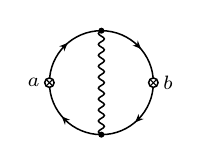
\begin{tikzpicture}[x=0.600cm, y=0.600cm, line width=0.550pt, baseline={([yshift=-0.6ex]0,0)}]
  \draw (0.000,-1.100) arc[start angle=270.000, end angle=180.000, radius=1.100];
  \fill (-0.840,-0.715) -- (-0.769,-0.894) -- (-0.756,-0.800) -- (-0.662,-0.787) -- cycle;
  \draw (0.000,1.100) arc[start angle=90.000, end angle=0.000, radius=1.100];
  \fill (0.840,0.715) -- (0.769,0.894) -- (0.756,0.800) -- (0.662,0.787) -- cycle;
  \draw (1.100,0.000) arc[start angle=0.000, end angle=-90.000, radius=1.100];
  \fill (0.715,-0.840) -- (0.894,-0.769) -- (0.800,-0.756) -- (0.787,-0.662) -- cycle;
  \draw (-1.100,0.000) arc[start angle=180.000, end angle=90.000, radius=1.100];
  \fill (-0.715,0.840) -- (-0.894,0.769) -- (-0.800,0.756) -- (-0.787,0.662) -- cycle;
  \draw plot[smooth, tension=0.7] coordinates {(0.000,-1.100) (-0.044,-1.071) (-0.063,-1.042) (-0.044,-1.013) (0.000,-0.984) (0.044,-0.955) (0.063,-0.926) (0.044,-0.897) (0.000,-0.868) (-0.044,-0.839) (-0.063,-0.811) (-0.044,-0.782) (0.000,-0.753) (0.044,-0.724) (0.063,-0.695) (0.044,-0.666) (0.000,-0.637) (-0.044,-0.608) (-0.063,-0.579) (-0.044,-0.550) (0.000,-0.521) (0.044,-0.492) (0.063,-0.463) (0.044,-0.434) (0.000,-0.405) (-0.044,-0.376) (-0.063,-0.347) (-0.044,-0.318) (0.000,-0.289) (0.044,-0.261) (0.063,-0.232) (0.044,-0.203) (0.000,-0.174) (-0.044,-0.145) (-0.063,-0.116) (-0.044,-0.087) (0.000,-0.058) (0.044,-0.029) (0.063,0.000) (0.044,0.029) (0.000,0.058) (-0.044,0.087) (-0.063,0.116) (-0.044,0.145) (0.000,0.174) (0.044,0.203) (0.063,0.232) (0.044,0.261) (0.000,0.289) (-0.044,0.318) (-0.063,0.347) (-0.044,0.376) (0.000,0.405) (0.044,0.434) (0.063,0.463) (0.044,0.492) (0.000,0.521) (-0.044,0.550) (-0.063,0.579) (-0.044,0.608) (0.000,0.637) (0.044,0.666) (0.063,0.695) (0.044,0.724) (0.000,0.753) (-0.044,0.782) (-0.063,0.811) (-0.044,0.839) (0.000,0.868) (0.044,0.897) (0.063,0.926) (0.044,0.955) (0.000,0.984) (-0.044,1.013) (-0.063,1.042) (-0.044,1.071) (0.000,1.100)};
  \draw[fill=white] (-1.100,0.000) circle (0.100);
  \draw[line width=0.390pt] (-1.030,0.070) -- (-1.170,-0.070) (-1.030,-0.070) -- (-1.170,0.070);
  \draw[fill=white] (1.100,0.000) circle (0.100);
  \draw[line width=0.390pt] (1.170,0.070) -- (1.030,-0.070) (1.170,-0.070) -- (1.030,0.070);
  \fill (0.000,-1.100) circle (0.064);
  \fill (0.000,1.100) circle (0.064);
  \node[font=\scriptsize, inner sep=0pt, anchor=0] at (-1.290,0.000) {$a$};
  \node[font=\scriptsize, inner sep=0pt, anchor=180] at (1.290,0.000) {$b$};
\end{tikzpicture}
\allowbreak\;{+}\; 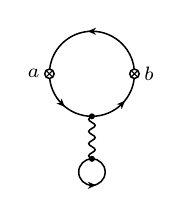
\begin{tikzpicture}[x=0.600cm, y=0.600cm, line width=0.550pt, baseline={([yshift=-0.6ex]0,0)}]
  \draw (0.900,0.000) arc[start angle=0.000, end angle=180.000, radius=0.900];
  \fill (-0.089,0.900) -- (0.089,0.824) -- (0.031,0.900) -- (0.089,0.976) -- cycle;
  \draw (0.000,-0.900) arc[start angle=270.000, end angle=360.000, radius=0.900];
  \fill (0.699,-0.574) -- (0.520,-0.646) -- (0.614,-0.658) -- (0.627,-0.753) -- cycle;
  \draw (-0.900,0.000) arc[start angle=180.000, end angle=270.000, radius=0.900];
  \fill (-0.574,-0.699) -- (-0.646,-0.520) -- (-0.658,-0.614) -- (-0.753,-0.627) -- cycle;
  \draw plot[smooth, tension=0.7] coordinates {(0.000,-1.800) (-0.049,-1.768) (-0.069,-1.736) (-0.049,-1.704) (0.000,-1.671) (0.049,-1.639) (0.069,-1.607) (0.049,-1.575) (0.000,-1.543) (-0.049,-1.511) (-0.069,-1.479) (-0.049,-1.446) (0.000,-1.414) (0.049,-1.382) (0.069,-1.350) (0.049,-1.318) (0.000,-1.286) (-0.049,-1.254) (-0.069,-1.221) (-0.049,-1.189) (0.000,-1.157) (0.049,-1.125) (0.069,-1.093) (0.049,-1.061) (0.000,-1.029) (-0.049,-0.996) (-0.069,-0.964) (-0.049,-0.932) (0.000,-0.900)};
  \draw (0.000,-1.800) arc[start angle=90.000, end angle=450.000, radius=0.280];
  \fill (0.089,-2.360) -- (-0.089,-2.284) -- (-0.031,-2.360) -- (-0.089,-2.436) -- cycle;
  \draw[fill=white] (-0.900,0.000) circle (0.100);
  \draw[line width=0.390pt] (-0.830,0.070) -- (-0.970,-0.070) (-0.830,-0.070) -- (-0.970,0.070);
  \draw[fill=white] (0.900,0.000) circle (0.100);
  \draw[line width=0.390pt] (0.970,0.070) -- (0.830,-0.070) (0.970,-0.070) -- (0.830,0.070);
  \fill (0.000,-1.800) circle (0.064);
  \fill (0.000,-0.900) circle (0.064);
  \node[font=\scriptsize, inner sep=0pt, anchor=0] at (-1.090,0.001) {$a$};
  \node[font=\scriptsize, inner sep=0pt, anchor=180] at (1.090,0.001) {$b$};
\end{tikzpicture}
\allowbreak\;{-}\; 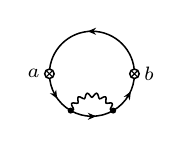
\begin{tikzpicture}[x=0.600cm, y=0.600cm, line width=0.550pt, baseline={([yshift=-0.6ex]0,0)}]
  \draw (0.900,0.000) arc[start angle=0.000, end angle=180.000, radius=0.900];
  \fill (-0.089,0.900) -- (0.089,0.824) -- (0.031,0.900) -- (0.089,0.976) -- cycle;
  \draw (0.450,-0.779) arc[start angle=300.000, end angle=360.000, radius=0.900];
  \fill (0.824,-0.373) -- (0.670,-0.489) -- (0.764,-0.477) -- (0.801,-0.565) -- cycle;
  \draw (-0.450,-0.779) arc[start angle=240.000, end angle=300.000, radius=0.900];
  \fill (0.089,-0.900) -- (-0.089,-0.824) -- (-0.031,-0.900) -- (-0.089,-0.976) -- cycle;
  \draw plot[smooth, tension=0.7] coordinates {(0.450,-0.779) (0.411,-0.769) (0.390,-0.755) (0.394,-0.730) (0.414,-0.695) (0.431,-0.658) (0.429,-0.629) (0.404,-0.617) (0.362,-0.619) (0.322,-0.625) (0.298,-0.620) (0.292,-0.595) (0.297,-0.555) (0.299,-0.514) (0.286,-0.488) (0.258,-0.487) (0.221,-0.505) (0.186,-0.525) (0.161,-0.529) (0.146,-0.509) (0.136,-0.470) (0.122,-0.431) (0.100,-0.412) (0.074,-0.422) (0.046,-0.452) (0.021,-0.484) (0.000,-0.498) (-0.021,-0.484) (-0.046,-0.452) (-0.074,-0.422) (-0.100,-0.412) (-0.122,-0.431) (-0.136,-0.470) (-0.146,-0.509) (-0.161,-0.529) (-0.186,-0.525) (-0.221,-0.505) (-0.258,-0.487) (-0.286,-0.488) (-0.299,-0.514) (-0.297,-0.555) (-0.292,-0.595) (-0.298,-0.620) (-0.322,-0.625) (-0.362,-0.619) (-0.404,-0.617) (-0.429,-0.629) (-0.431,-0.658) (-0.414,-0.695) (-0.394,-0.730) (-0.390,-0.755) (-0.411,-0.769) (-0.450,-0.779)};
  \draw (-0.900,0.000) arc[start angle=180.000, end angle=240.000, radius=0.900];
  \fill (-0.735,-0.527) -- (-0.758,-0.335) -- (-0.795,-0.423) -- (-0.889,-0.411) -- cycle;
  \draw[fill=white] (-0.900,0.000) circle (0.100);
  \draw[line width=0.390pt] (-0.830,0.070) -- (-0.970,-0.070) (-0.830,-0.070) -- (-0.970,0.070);
  \draw[fill=white] (0.900,0.000) circle (0.100);
  \draw[line width=0.390pt] (0.970,0.070) -- (0.830,-0.070) (0.970,-0.070) -- (0.830,0.070);
  \fill (0.450,-0.779) circle (0.064);
  \fill (-0.450,-0.779) circle (0.064);
  \node[font=\scriptsize, inner sep=0pt, anchor=359] at (-1.090,0.002) {$a$};
  \node[font=\scriptsize, inner sep=0pt, anchor=181] at (1.090,0.002) {$b$};
\end{tikzpicture}
\allowbreak\;{+}\; 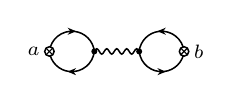
\begin{tikzpicture}[x=0.600cm, y=0.600cm, line width=0.550pt, baseline={([yshift=-0.6ex]0,0)}]
  \draw (-0.475,0.000) arc[start angle=353.974, end angle=186.026, radius=0.478];
  \fill (-1.039,-0.427) -- (-0.861,-0.503) -- (-0.919,-0.427) -- (-0.861,-0.352) -- cycle;
  \draw (-1.425,0.000) arc[start angle=173.974, end angle=6.026, radius=0.478];
  \fill (-0.861,0.427) -- (-1.039,0.503) -- (-0.981,0.427) -- (-1.039,0.352) -- cycle;
  \draw (0.475,0.000) arc[start angle=186.026, end angle=353.974, radius=0.478];
  \fill (1.039,-0.428) -- (0.861,-0.352) -- (0.919,-0.428) -- (0.861,-0.503) -- cycle;
  \draw (1.425,0.000) arc[start angle=6.026, end angle=173.974, radius=0.478];
  \fill (0.861,0.428) -- (1.039,0.352) -- (0.981,0.428) -- (1.039,0.503) -- cycle;
  \draw plot[smooth, tension=0.7] coordinates {(-0.475,0.000) (-0.449,0.040) (-0.422,0.057) (-0.396,0.040) (-0.369,0.000) (-0.343,-0.040) (-0.317,-0.057) (-0.290,-0.040) (-0.264,0.000) (-0.238,0.040) (-0.211,0.057) (-0.185,0.040) (-0.158,0.000) (-0.132,-0.040) (-0.106,-0.057) (-0.079,-0.040) (-0.053,0.000) (-0.026,0.040) (0.000,0.057) (0.026,0.040) (0.053,0.000) (0.079,-0.040) (0.106,-0.057) (0.132,-0.040) (0.158,0.000) (0.185,0.040) (0.211,0.057) (0.237,0.040) (0.264,0.000) (0.290,-0.040) (0.317,-0.057) (0.343,-0.040) (0.369,0.000) (0.396,0.040) (0.422,0.057) (0.449,0.040) (0.475,0.000)};
  \draw[fill=white] (-1.425,0.000) circle (0.100);
  \draw[line width=0.390pt] (-1.355,0.070) -- (-1.495,-0.070) (-1.355,-0.070) -- (-1.495,0.070);
  \draw[fill=white] (1.425,0.000) circle (0.100);
  \draw[line width=0.390pt] (1.495,0.070) -- (1.355,-0.070) (1.495,-0.070) -- (1.355,0.070);
  \fill (-0.475,0.000) circle (0.064);
  \fill (0.475,0.000) circle (0.064);
  \node[font=\scriptsize, inner sep=0pt, anchor=0] at (-1.615,0.000) {$a$};
  \node[font=\scriptsize, inner sep=0pt, anchor=180] at (1.615,0.000) {$b$};
\end{tikzpicture}
\allowbreak\;{+}\; 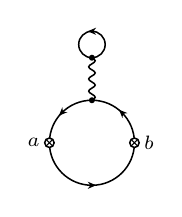
\begin{tikzpicture}[x=0.600cm, y=0.600cm, line width=0.550pt, baseline={([yshift=-0.6ex]0,0)}]
  \draw (0.000,0.900) arc[start angle=90.000, end angle=180.000, radius=0.900];
  \fill (-0.699,0.574) -- (-0.520,0.646) -- (-0.614,0.658) -- (-0.627,0.753) -- cycle;
  \draw (-0.900,0.000) arc[start angle=180.000, end angle=360.000, radius=0.900];
  \fill (0.089,-0.900) -- (-0.089,-0.824) -- (-0.031,-0.900) -- (-0.089,-0.976) -- cycle;
  \draw (0.900,0.000) arc[start angle=0.000, end angle=90.000, radius=0.900];
  \fill (0.574,0.699) -- (0.646,0.520) -- (0.658,0.614) -- (0.753,0.627) -- cycle;
  \draw plot[smooth, tension=0.7] coordinates {(0.000,1.800) (0.049,1.768) (0.069,1.736) (0.049,1.704) (0.000,1.671) (-0.049,1.639) (-0.069,1.607) (-0.049,1.575) (0.000,1.543) (0.049,1.511) (0.069,1.479) (0.049,1.446) (0.000,1.414) (-0.049,1.382) (-0.069,1.350) (-0.049,1.318) (0.000,1.286) (0.049,1.254) (0.069,1.221) (0.049,1.189) (0.000,1.157) (-0.049,1.125) (-0.069,1.093) (-0.049,1.061) (0.000,1.029) (0.049,0.996) (0.069,0.964) (0.049,0.932) (0.000,0.900)};
  \draw (0.000,1.800) arc[start angle=270.000, end angle=630.000, radius=0.280];
  \fill (-0.089,2.360) -- (0.089,2.284) -- (0.031,2.360) -- (0.089,2.436) -- cycle;
  \draw[fill=white] (-0.900,0.000) circle (0.100);
  \draw[line width=0.390pt] (-0.830,0.070) -- (-0.970,-0.070) (-0.830,-0.070) -- (-0.970,0.070);
  \draw[fill=white] (0.900,0.000) circle (0.100);
  \draw[line width=0.390pt] (0.970,0.070) -- (0.830,-0.070) (0.970,-0.070) -- (0.830,0.070);
  \fill (0.000,1.800) circle (0.064);
  \fill (0.000,0.900) circle (0.064);
  \node[font=\scriptsize, inner sep=0pt, anchor=0] at (-1.090,-0.001) {$a$};
  \node[font=\scriptsize, inner sep=0pt, anchor=180] at (1.090,-0.001) {$b$};
\end{tikzpicture}
\allowbreak\;{-}\; 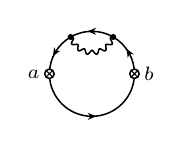
\begin{tikzpicture}[x=0.600cm, y=0.600cm, line width=0.550pt, baseline={([yshift=-0.6ex]0,0)}]
  \draw (-0.450,0.779) arc[start angle=120.000, end angle=180.000, radius=0.900];
  \fill (-0.824,0.373) -- (-0.670,0.489) -- (-0.764,0.477) -- (-0.801,0.565) -- cycle;
  \draw (-0.900,0.000) arc[start angle=180.000, end angle=360.000, radius=0.900];
  \fill (0.089,-0.900) -- (-0.089,-0.824) -- (-0.031,-0.900) -- (-0.089,-0.976) -- cycle;
  \draw (0.450,0.779) arc[start angle=60.000, end angle=120.000, radius=0.900];
  \fill (-0.089,0.900) -- (0.089,0.824) -- (0.031,0.900) -- (0.089,0.976) -- cycle;
  \draw plot[smooth, tension=0.7] coordinates {(-0.450,0.779) (-0.411,0.769) (-0.390,0.755) (-0.394,0.730) (-0.414,0.695) (-0.431,0.658) (-0.429,0.629) (-0.404,0.617) (-0.362,0.619) (-0.322,0.625) (-0.298,0.620) (-0.292,0.595) (-0.297,0.555) (-0.299,0.514) (-0.286,0.488) (-0.258,0.487) (-0.221,0.505) (-0.186,0.525) (-0.161,0.529) (-0.146,0.509) (-0.136,0.470) (-0.122,0.431) (-0.100,0.412) (-0.074,0.422) (-0.046,0.452) (-0.021,0.484) (0.000,0.498) (0.021,0.484) (0.046,0.452) (0.074,0.422) (0.100,0.412) (0.122,0.431) (0.136,0.470) (0.146,0.509) (0.161,0.529) (0.186,0.525) (0.221,0.505) (0.258,0.487) (0.286,0.488) (0.299,0.514) (0.297,0.555) (0.292,0.595) (0.298,0.620) (0.322,0.625) (0.362,0.619) (0.404,0.617) (0.429,0.629) (0.431,0.658) (0.414,0.695) (0.394,0.730) (0.390,0.755) (0.411,0.769) (0.450,0.779)};
  \draw (0.900,0.000) arc[start angle=360.000, end angle=420.000, radius=0.900];
  \fill (0.735,0.527) -- (0.758,0.335) -- (0.795,0.423) -- (0.889,0.411) -- cycle;
  \draw[fill=white] (-0.900,0.000) circle (0.100);
  \draw[line width=0.390pt] (-0.830,0.070) -- (-0.970,-0.070) (-0.830,-0.070) -- (-0.970,0.070);
  \draw[fill=white] (0.900,0.000) circle (0.100);
  \draw[line width=0.390pt] (0.970,0.070) -- (0.830,-0.070) (0.970,-0.070) -- (0.830,0.070);
  \fill (-0.450,0.779) circle (0.064);
  \fill (0.450,0.779) circle (0.064);
  \node[font=\scriptsize, inner sep=0pt, anchor=1] at (-1.090,-0.002) {$a$};
  \node[font=\scriptsize, inner sep=0pt, anchor=179] at (1.090,-0.002) {$b$};
\end{tikzpicture}